\documentclass{ieeeaccess}
\usepackage{cite}
\usepackage{amsmath,amssymb,amsfonts}
\usepackage{algorithmic}
\usepackage{graphicx}
\usepackage{textcomp}
\usepackage{lscape}
\usepackage{lineno,hyperref,longtable}
\usepackage{multirow}

\def\BibTeX{{\rm B\kern-.05em{\sc i\kern-.025em b}\kern-.08em
    T\kern-.1667em\lower.7ex\hbox{E}\kern-.125emX}}
\begin{document}
\history{Date of publication xxxx 00, 0000, date of current version xxxx 00, 0000.}
\doi{10.1109/ACCESS.2017.DOI}

\title{The state of big data reference architectures: a
systematic literature review}

\author{\uppercase{Pouya Ataei}\authorrefmark{1},
\uppercase{Alan Litchfield} \authorrefmark{2}.}

\address[1]{School of Engineering, Computer and Mathematical Sciences, Auckland University of Technology, Auckland, New Zealand (e-mail: pouya.ataei@aut.ac.nz)}

\address[2]{Service and Cloud Computing Research Lab, Auckland University of Technology, Auckland, New Zealand (e-mail: alan.litchfield@aut.ac.nz)}

\begin{abstract}
    Big Data (BD) is a nascent term emerged to describe large amount of data that comes in different forms from various channels. In modern world, users are the ceaseless generators of structured, semi-structured, and unstructured data that if gleaned and crunched precisely, will reveal game-changing patterns. While the opportunities exist with BD, the unprecedented amount of data has brought traditional approaches to a bottleneck, and the growth of data is outpacing technological and scientific advances in data analytics. It is estimated that approximately 75\% of the BD projects have failed within the last decade according to multiple sources. Among the challenges, system development and data architecture are prominent. This paper aims to facilitate BD system development and architecture by conducting a systematic literature review on BD reference architectures (RA). The primary goal is to highlight the state of BD RAs and how they can be helpful for BD system development. The secondary goal is to find all BD RAs, describe the challenges of creating these RA, discuss the common architectural components of these RA and the limitations of these RA. As a result of this work, firstly major concepts about RA are discussed and their applicability to BD system development is depicted. Secondly, 22 BD reference architecture is assessed from academia and practice and their commonalities, challenges, and limitations are identified. The findings gained emerges the understanding that RAs can be an effective artefact to tackle complex BD system development.
\end{abstract}

\begin{keywords}
    Big Data, Big Data Reference Architectures, Big Data Architectures, Big Data for business, Data analytics, Data engineering, Data-intensive applications, Reference Architectures
\end{keywords}

\titlepgskip=-15pt

\maketitle

\section{Introduction}

The rapid development of software technologies, the proliferation of digital devices and networking infrastructure of today, have by and large, augmented user’s capability to generate data \cite{AtaeiSecurity}. In the age of information, users are unceasing generators of structured, semi-structured, and unstructured data that if collected and crunched correctly, may reveal game-changing patterns \cite{AtaeiACIS}.

The unprecedented proliferation of data have emerged a new ecosystem of technologies; one of these ecosystems is BD \cite{AtaeiHype}. BD is a term emerged to describe large amount of data that comes in various forms from different channels. Within the years, BD has attained a lot of attention from academia and industry, and many strive to benefit from this new material. Howbeit, adopting BD requires the absorption of great deal of complexity and many traditional systems cannot cope with characteristics of this domain. 

A recent survey published by Databricks in partnership with MIT Technology Review Insights, stated that only 13\% of companies excel at delivering on their data strategy \cite{DataBricksSurvey}. In the same vein, Vintage Partners highlighted that only 24\% of companies have successfully adopted BD \cite{NewVantageSurvey}. Sigma computing report presented that 1 in 4 business experts have given up on getting insights they needed because the data processing took too long \cite{SigmaSurvey}. Moreover, Gartner approximated that only 20\% of companies have successfully adopted BD. 

Some of the most highlighted challenges of BD is 'lack of business context', 'organizational challenges', 'BD architecture', 'data engineering', 'rapid technology change', and 'lack of talent' \cite{AtaeiBigDataEnvirons}. Whereas similar issues may exist in other domains, it is exacerbated when it comes to BD systems. This is due the inherent complexity of BD engineering, the need for real-time processing, the scalability requirement of these systems, and the sensitivities around data.

Today, majority of BD systems are designed underlying ad-hoc and complicated architectural solutions \cite{Gorton}, that do not seem to adhere to similar patterns. This will challenge software architects to design a suitable solution for any given context, creates a foundation for an immature architectural decision, and does not promote the growth and development of BD systems as a whole. 

Therefore, since the approach of ad-hoc design to BD systems is undesirable and leaves many engineers in the dark, there is a need for more software engineering research for BD systems. To this end, this study presents a systematic literature review (SLR) on BD (BD) reference architectures (RAs). 

\section{Why reference architectures?}
Conceptualization of the system as an RA, helps with understanding of the system’s key components, behavior, composition and evolution of it, which in turn affect quality attributes such as maintainability, scalability and performance \cite{Cloutier}. Therefore RAs can be a good standardization artefact and a communication medium that not only results in concrete architectures for BD systems, but also provide stakeholders with unified elements and symbols to discuss and progress BD projects.

This approach to system development is not new to practitioners of complex system. In software product line (SPL) development, RAs are utilized as generic artifacts that are instantiated and configured for a particular domain of systems \cite{Derras}. In software engineering, IT giants like IBM have referred to RAs as the 'best of best practices' to address complex and unique system design challenges \cite{Cloutier}. In other international standardization, RAs have been repeatedly used to standardize an emerging domain, a good example of this is BS ISO/IEC 18384-1 RA for service oriented architectures \cite{Iso18384-1}. 

\section{Reference Architectures State of the art}

Despite the benefits of utilizing RAs, and their potential to solve some of the complex issues of BD systems, we think that this area is underdeveloped and needs more attention from both academia and practice. This insight is derived from our preliminary systematic review in academia, and search for available big data RAs (\cite{AtaeiACIS}).

One of the most comprehensive BD RA published, is the National Institute of Standards and Technology (NIST) BD RA, which published by Big Data Public Working Group (NBD-PWG) with large set of contributors from academia, industry, non-profit organizations, and others. This RA was an initiative from White house in March 2012, and was published in October 2019 with considerable amount of investment. 

Given the substantial investment on BD RAs, one might infer the value of these artifacts, and this can in turn highlights the necessity for more research in this domain. Another factor that came to light, is how vaguely the phrase 'reference architecture' is defined and institutionalized. For instance, the difference between a 'concrete architecture' and a 'reference architecture' is hardly discussed, and different domains seem to have defined the artifact slightly differently. 

For instance, Cloutier et al (\cite{Cloutier}) presented that 'Reference Architectures capture the essence of existing architectures, and the vision of future needs and evolution to provide guidance to assist in developing new system architectures'. This definition is derived from the system engineering domain and by the means of collaborative forum from Steven's institute of technology. In another effort, Muller et al (\cite{muller2008reference}) defines RA as 'artifacts that captures the essence of architecture of a collection of systems'. This definition is driven from the product line engineering domain. 

In the same vein, Angelov et al (\cite{angelov2009classification}) proposed that 'A reference architecture is a generic architecture for a class of information systems that is used as a foundation for the design of concrete architectures in this class'. Another definition by Bass et al (\cite{Bass}) stated that 'A reference architecture is a reference model mapped onto software elements (that cooperatively implement the functionality defined in the reference model) and the data flows between them'. 

Although different authors may have defined RAs in different ways, the essence remains the same: to reuse the software engineering knowledge for a class of systems, particularly in relation to architecture. Moreover, the difference between RAs and concrete architectures is rarely discussed. 

\section{Objective of the study}

Given the failure rate of BD projects, we posit RAs as potential solution to facilitate system development and BD architecture, and aim to explore this area through a systematic literature review. Up to date, there's only one SLR that explored this area (\cite{AtaeiACIS}), which is outdated, suffers from methodological clarity, and is published as a conference paper, which implies lack of detail.

Based on this, the objective of this review is to find and collate the BD RAs available from the body of evidence, highlight their architectural commonality and point out the limitations. This study can be considered a useful primer for practitioners or academics who are interested in adopting BD. 

The research questions are formulated as the following; 
\begin{enumerate}
    \item \textbf{RQ1}: What are current BD RAs available in academia and industry?
    \item \textbf{RQ2}: What are major architectural components of these BD RAs? 
    \item \textbf{RQ3}: What are the limitations of current BD RAs?
\end{enumerate}

We found these questions relevant to our study firstly because they address a gap in the body of knowledge (BD RAs), secondly because they aim to capture the essence of practice on architecting big data systems and lastly because they shed lights on limitations of current BD RAs and common choke points. 

\section{Review Methodology:}
This research follows the guidelines of PRISMA (\cite{page2021prisma}). In addition, we adopted PRISMA-S (\cite{rethlefsen2021prisma}) to improve our search strategy and lastly we have used Barbara et al's guidelines for evidence based software engineering and systematic reviews \cite{kitchenham2015evidence}. Although PRISMA is a comprehensive guidelines on conducting a systematic literature review, it is derived from the healthcare community and is driven by assumptions that may not be thoroughly relevant to software engineering and information system researchers. To this end, Barbara et al \cite{kitchenham2015evidence} has translated many of these assumptions to the domain of software engineering and included many guidelines for lone researchers and projects with small number of researchers.

We have therefore utilized PRISMA as the underpinning of our research design, with complementary studies to reduce bias, improve transparency and systematiticity. SLR has been chosen because it is a qualitative research methodology that is aimed at driving knowledge and understanding about an emerging topic and the elements surrounding it. Besides, SLR provides a transparent and reproducible procedure that elicits patterns, relationships, trends, and delineates the overall picture of the subject \cite{borrego2014systematic}.

The main objective of this study is to assess the current state of BD RAs, identify their major architectural components, point out fundamental concepts and discuss their limitations. This objective is achieved in four phases. In first phase, research questions are stated, exclusion and inclusion criteria are defined, literature are identified and pooled, and the quality framework is developed. In second phase, the title of the studies are assessed based on the inclusion and exclusion criteria. After that, the filtered studies are once more assessed based on their title, abstract, introduction and conclusion. After this, full analysis of the studies took place by running each study against the criteria defined in the quality framework. Thirdly, selected pool of literature is coded based on research questions. Lastly, findings are synthesized by the means of thematic synthesis, and themes realized are depicted.

This study builds on the SLR conducted by Ataei et al \cite{AtaeiACIS} and aims to improve it by covering the years 2020 to 2022. Unlike Ataei's work, this paper aims to employ thematic synthesis, and provide a more detailed view of BD RAs and their properties.

\subsection{Identification}

The first phase of the SLR began, by adoption of PRISMA-S (\cite{rethlefsen2021prisma}) to develop a robust multi-database search strategy. This extension of PRISMA provided us with a framework of 12 items to increase transparency, systematiticity, and reduce bias in our search strategy. For the purposes of this study, following electronic databases were searched: ScienceDirect, IEEE Explore, SpringerLink, AISeL, JSTOR and ACM library. To pursue to goal of finding all literature available on the topic, and to avoid overlooking valuable research, abstract and citation databases and search engines such as Google Scholar, and Research Gate was used.

We also searched the grey literature on the topic, using the search string "big data" AND "reference architecture*" on Google ( in June 2022 ). The first 40 results were selected for screening. This was done in 'incognito mode' to avoid any personal customization of the google search pages. Reference lists of included studies were manually screened to identify additional studies. This is to achieve the critical component of 'completeness' for SLRs, as suggested by Kitchenham et al \cite{kitchenham2015evidence}.

The platform search capabilities varied, but our search strategy remained uniform for most parts. For instance, if a platform did not support wildcards ( like asterisk ), we just searched twice for the singular and plural version of the word. The only exception that made the selection process longer was SpringerLink, because it did not support bulk download of references in BibTex format. The keywords for the chosen databases are as following: 

\begin{itemize}
    \item ("Document Title":big data) AND ("Document Title":reference architecture) OR ("Document Title":big data architecture)
\end{itemize}

The reason we included architecture is due to the fact that, terms \emph{reference architecture} and \emph{architecture} may have been used interchangeably, and an architecture that is at the abstraction level of an RA, might have been called just an architecture. Therefore it was critical for us to firmly define these terms and then categorize studies based on these definitions. These definitions and our findings are depicted in the findings section.

Our initial search was limited to year 2020 to year 2022, as the work of Ataei et al \cite{AtaeiACIS} covered the years 2010-2020. Nevertheless, we still included the years 2010 to 2020 to make sure no research is left out or overlooked. This implies that even though our work is derived from Ataei et al \cite{AtaeiACIS} study, we still have done a complete SLR to cover all the years on the topic. These years are chosen firstly because more contemporary researches are focused on the facilitation of big data system development, and secondly there's no SLR that has covered these years for BD RAs.

To achieve these limits, we have utilized databases features. All databases supported the selection of year range, and the language limit was automatically applied by doing an advanced search with the aforementioned keywords.

Our approach to systematic collection of evidence was to search databases using the keywords aforementioned and then bulk download the BibTex files. Majority of the databases supported bulk downloading of BibTex files except for SpringerLink, Google Scholar, and Research Gate. For SpringerLink we downloaded the studies in CSV format and then converted them to BibTex using a custom script. For Google Scholar and ResearchGate, unfortunately, we had to take the manual path of creating a bib file for the studies. 

Once all the bib files have been created, we merged them into one large bib file and imported it to a software called JabRef (\cite{JabRef}) for deduplication. 172 studies are pooled initially, out of which 6 duplicates have been identified. We removed the primary SLR that this study is based on, and also another paper that we could not find the citation for. In the other extreme, we found 5 white papers and 4 website blogs and added them to the selection pool. At the end of this phase, 173 studies have been pooled. 

\subsection{Screening and Eligibility}

Stage 1 of screening started with assessing the title, abstract, and keywords of the pooled studies. For grey literatures simply the title. This was achieved based on our inclusion and exclusion criteria. The inclusion criteria are as following;

\begin{itemize}
    \item Primary and secondary studies (including grey literature) between Jan 1st 2010 and June 1st 2022 on the topics of BD RA, BD architecture, and BD architectural components were included. 
    \item Research that Indicates the current state of RAs in the field of BD and demonstrates possible outcomes
    \item Studies that are scholarly publications, books, book chapters, thesis, dissertations, or conference proceedings 
    \item Grey literature such as white paper that includes extensive information on BD RAs
\end{itemize}

And the studies with the following topics were excluded: 

\begin{itemize}
    \item Informal literature surveys without any clearly defined research questions or research process
    \item Duplicate reports of the same study (a conference and journal version of the same paper)
    \item Short papers (less than 5 pages)
    \item Studies that are not written in English
\end{itemize}

Disagreement among researchers were resolved using Krippendorff’s alpha (\cite{krippendorff2011computing}). Our aim was not to get involved in a very complicated statistics model, so we've done most of the computations using SPSS, specifically with Hayes’ Macro. We made sure that a separate file is created for each variable, and inserted coders as variables and not a constant value. Our $ \alpha $ value was within the acceptable range (above 80), and any disagreement was solved by inviting a third person or a moderator. When $ \alpha $ value was very low (indicating a low reliability), we stopped the process, and tried to clarify fundamental concepts and categories. The final computed $ \alpha $ value was 89.9\%. 

In stage 2, After excluding papers based on inclusion and exclusion criteria, and as suggested by Kitchenham et al \cite{kitchenham2015evidence}, we assessed studies based on their quality. Quality of the evidence collected as a result of this SLR has direct impact on the quality of the findings, making quality assessment an important undertaking.

However, this process comes with some well-known complexities. The most fundamental ones are, perhaps defining the term 'quality', and secondly trying to appraise the quality of conference papers that rarely provide enough detail on research methodology and evaluation. Generally, a quality of a study is tightly associated to its research method and the validity of its findings. From this perspective, and inspired by the works of Noblit and Hare on meta-ethnography (\cite{noblit1988meta}), and Dyba et al (\cite{dybaa2008empirical}), quality of studies is assessed by the extent to which the conduct, design and analysis of a research is susceptible to systematic errors or bias (\cite{cumpston2019updated}). That is, the more bias in the selected literature, the more chance to create miss-leading conclusions.

Considering the rather heterogeneous nature of software engineering and information systems (IS) papers, and difficulty of defining quality in studies with varying nature, we first analyzed a few well-established checklists such as Critical Appraisal Skills Programme (CASP \cite{tools2018checklists}), and JBI's critical appraisal tool (\cite{JBI}). Whereas these checklists could potentially account for the requirements of this study, we opted for something that is more specific to software engineering and IS. We realized for example that, Runeson et al (\cite{runeson2006we}) provided a checklist designated to help researchers reading and undertaking software engineering case studies. In the same vein, Dyba et al (\cite{dybaa2008empirical}) proposed a quality criteria based on CASP checklist for qualitative studies in software engineering systematic reviews. 

Nevertheless, the challenge is that our study includes a large number of different study types that needs to go through a single checklist. To address this, we developed a criteria made up of 7 elements. These criteria are informed by those proposed by CASP for assessing the quality of qualitative research (\cite{tools2018checklists}) and by guidelines provided by Kitchenham (\cite{kitchenham2002preliminary}) on empirical research in software engineering. The 7 criteria tested literature on 4 major areas that can critically affect the quality of the studies. These categories and the corresponding criteria are as following;

\begin{enumerate}
    \item \emph{Minimum quality threshold:} 
    \begin{enumerate}
        \item Does the study report empirical research or is it merely a 'lesson learnt' report based on expert opinion ?
        \item The objectives and aims of the study is clearly communicated, including the reasoning for why the study was undertaken ? 
        \item Does the study provide with adequate information regarding the context in which the research was carried out ?
    \end{enumerate}
    \item \emph{Rigour:}
    \begin{enumerate}
        \item Is the research design appropriate to address the objectives of the research ?
        \item Is there any data collection method used and is it appropriate ?
    \end{enumerate}
    \item \emph{Credibility:}
      \begin{enumerate}
        \item Does the study report findings in a clear and unbiased manner ? 
     \end{enumerate}
    \item \emph{Relevance:}
    \begin{enumerate}
        \item Does the study provides value for practice or research 
     \end{enumerate}
\end{enumerate}

Taken all together, these 7 criteria gave us a measure of the extent to which a particular study's findings could make a valuable contribution to the review. These criteria was disseminated as a checklist among researchers with value for each property being dichotomous, that is 'yes' or 'no' in two phases. In the first phase, researchers only assess the quality based on the first major area ( minimum quality threshold ). If the study passed the first phase, it would then go into the second phase, where it was assessed for credibility, rigour and relevance. The quality is agreed if 75\% of the responses are positive for any given study with at least 75\% inter-rater reliability. 

Disagreements regarding the quality was usually resolved through a meeting. While, the meeting could not address the disagreements, a moderator has been invited to the process. Lastly, it is worth mentioning that this quality framework was not used for grey literature. Grey literature were only assessed through inclusion and exclusion criteria. 

In the first phase (identification) of this SLR, a total of 138 literature has been pooled from academia, and 24 from grey literature. Some of this literature has been added to the pool by the process of forward and backward searching. For instance, by reading NIST RA, we found out about Oracle, Facebook, and Amazon RAs and included those in the pool of the literature as well. 

In the screening phase, the literature that were not in-line with our inclusion and exclusion criteria have been eliminated. For example, if the paper was very short and was not on the topic of BD RA, or its ecosystem or limitations, it was excluded. As a result of this phase, 50 papers excluded. In the next phase, by assessing studies against the quality framework, 21 studies from academia, and 12 studies from grey literature pool has been eliminated. The flowchart is depicted in figure ~\ref{fig:PRISMA}.


\begin{figure*}[t]
    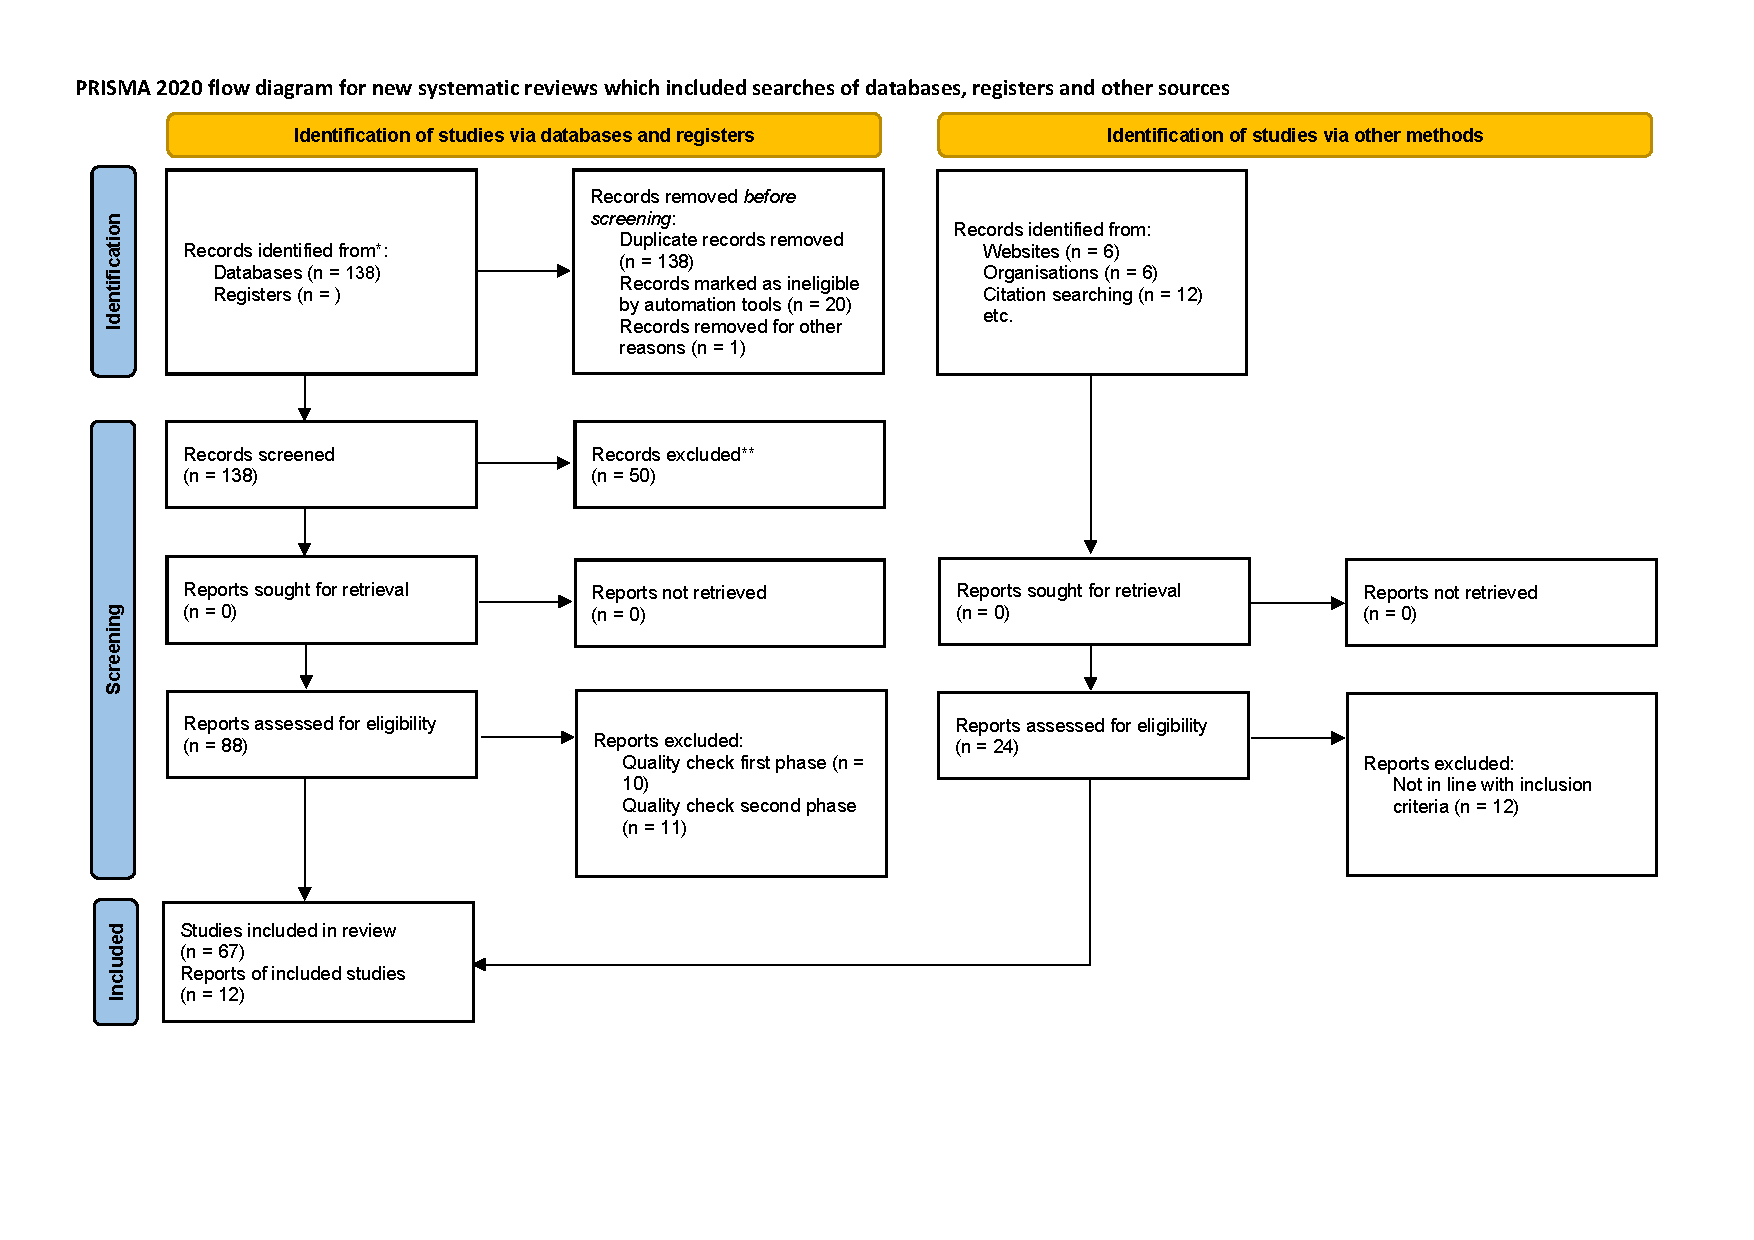
\includegraphics[width=18cm]{PRISMA/PRISMA_Flow_Diagram-2.pdf}
    \caption{PRISMA flowchart}
    \label{fig:PRISMA}
\end{figure*}


By the result of this work, 79 studies have been selected comprising of proceedings, journal articles, book chapters, and white papers. Out of the pool of articles, 33.3\% are from IEEE Explore, 5.2\% from ScienceDirect, 24.5\% from SpringerLink, 15.7\% from ACM, and 21\% from other sources such as Google Scholar, Research Gate and gray literature. 30 journal articles, 29 conference proceedings, 12 book chapters, 6 white papers, 1 Master’s Thesis and 1 PhD thesis were selected. 55\% of the articles were selected from the years 2016- 2022, 33\% belonged to years 2013-2016, and the rest to years 2010-2013. These stats are portrayed in figure \ref{fig:SLRStats}

\begin{figure*}[t]
    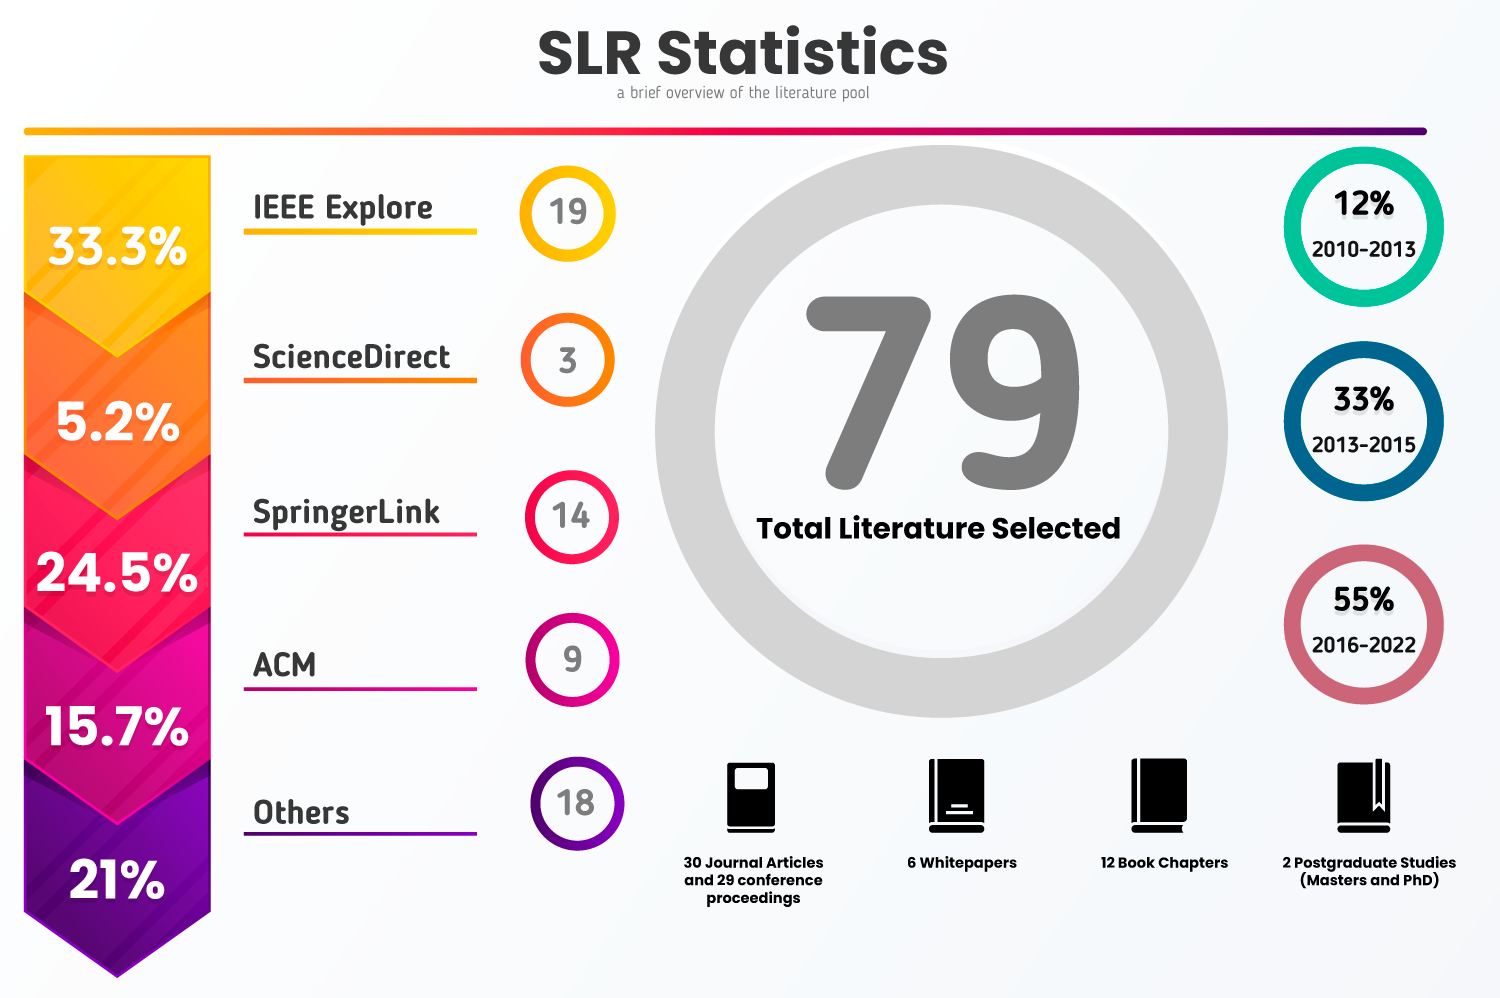
\includegraphics[width=18cm]{Media/databases-statitistic-[Recovered].png}
    \caption{SLR Statistics}
    \label{fig:SLRStats}
\end{figure*}

\subsection{Data Extraction and Synthesis}

By this stage, research questions have been set, inclusion and exclusion criteria are defined and applied, the quality assessment framework is developed and applied to the pool of studies, and the research embarked on actual synthesis of data. An integral element of this phase is data extraction, in which the essence of the studies are obtained in an explicit and consistent manner.

Precursor to synthesis of the actual data, we first followed the guidelines proposed by Dyba et al \cite{cruzes2011recommended} for data extraction. Data extraction firstly began by reading the entire pool of literature in order to get immersed with the data \cite{braun2006using}. From there on, we followed a structured reading approach and extracted three kind of data; 1) Publication Details (author, title, year, etc), 2) Contextual descriptions ( industry, settings, technologies ), and 3) Findings ( results, the actual RA, events, etc ..)

This process was a bit challenging, as some studies did not describe the method adequately, contextual information were not detailed often, and evaluation methods varied. To overcome this challenge, majority of this process took place in a consensus meeting \cite{dyba2007applying}.

After data extraction, we began the coding process. For this step, we've had several approaches ahead of us. Either we could adopt a deductive or a prior approach (\cite{miles1994qualitative}) or an inductive or grounded theory approach (\cite{corbin2014basics}). Neither of which could be as rigorous as we desired, thus we opted for an integrated approach (\cite{lofland1971analyzing}). We used the software Nvivo to organize our files and created an initial set of a priori codes based on research questions. These codes are as followings;

\begin{enumerate}
    \item BD RAs (RQ1)
    \item BD RAs Architectural components (RQ2)
    \item BD RAs limitations (RQ3)
\end{enumerate}

As the coding progressed, we realized that there is a need to define some of the fundamental areas that seem to not have been well established in academia and practice. For instance, we've been looking for studies that discuss the fundamental concepts of RAs. This was to further support our initiative, but we soon realized that this area is not standardized, and while there was mention of these concepts, they were usually lacking or were very short. Furthermore, not many studies discussed the benefits and relevance of RAs for BD systems. We also could not find a study that thoroughly discusses common approaches to developing BD RAs, and the challenges of developing a BD RA.

Based on these, therefore, we added the following extra four codes;
\begin{enumerate}
    \item Fundamental concepts of RAs
    \item How can RAs help BD system development
    \item Common approaches to creating BD RAs
    \item Challenges of creating BD RAs
\end{enumerate}

After having coded all the literature pooled, we began the process of turning them into themes. Themes helped us pull together segregated data into one meaningful whole that is above the sum of its constituents. This was not a single step process, and as we started to analyze codes, we have subsumed some first-cycle codes into higher-order codes. This also led to rearrangements and reclassification of the codes. The end of this process was marked, when the emerging themes saturated, and we could not derive a new theme. Many of the themes emerged have been then categorized into higher-order themes. 

The last step of data synthesis, was creation of a model based on the higher-order themes to explain relationships and to answer original research questions. The final product of this phase, is a theory, connection with prior theories, and indication of relationships. 

Of particular challenge we faced in this phase was the influence of heterogeneity, specifically given the inclusion of grey literature and cardinality of research methodologies in software engineering researches. Thus, to ensure the robustness of the higher-order themes we identified the main sources of variability as; 1) variability of outcomes ( some RAs well evaluated in practice, while some other are just compared against other RAs ), 2) variability in study designs ( methodological diversity that exists in software engineering and specifically in creation of RAs ), and 3) variability in study settings ( contextual factors are often not well reported ).

Last,but not least, to increase the rigour, we assessed the trustworthiness of the synthesis from three aspects; 1) Credibility: is the focus of the research in-line with research questions, and does the thematic synthesis cover data well ? 2) Conformability: are data extracted and coded in the correct way? do all researchers agree on this? would readers agree with the approach ? 3) Transferability: are the findings generalizable, can the findings be applied in different context? 

\section{Findings}

In this section, we map our findings against the research questions in a series of sub-sections. For increased clarity, these sub sections are driven by the research questions and models we created in the previous phase. We first begin by explaining fundamental concepts such as RAs and how they help BD system development (our inductive codes) and then progressively worked towards more specific topics such as current BD RAs and their limitations.

\subsection{What are the fundamental concepts of RAs?}

As the complexity of man-made systems grow, procedures, principles, and concepts of software architecture are increasingly applied to address those complexity faced by practitioners \cite{AtaeiACIS}. A system abstracted and expressed in terms of architectural concepts, facilitates the understanding of system’s essence, properties revolving around it, and evolution of it, which in turn affects quality attributes such as performance, maintainability, and scalability. 

In recent years, IT architectures played a pivotal role in the progress and evolution of system development and gained acceptance in maintenance, planning, development, and cost reduction of complex systems \cite{martinez2015solid}. To address ambiguity about what should be developed to address what needs, an architecture can play an overarching role by portraying the fundamental components of the system and the means and ways in which these components communicate to achieve the overall goal of the system \cite{Sievi-Korte}. This in turn creates manageable components that can be used to address different aspect of the problem and provides stakeholders with an abstract artefact to observe, reflect upon, contribute to, and communicate with \cite{kohler2019towards}

Many successful IT artefacts today stemmed from an effective RA. A few good examples are the Open Systems Interconnection model or OSI \cite{zimmermann1980osi}, Open Authentication or OATH \cite{OATH}, Common Object Request Broker Architecture or CORBA \cite{pope1998corba}, and WMS or workflow management systems \cite{greefhorst1999een}. In fact, every system goes with an architecture, either known or unknown, and it is in the architecture that the overall qualities of the system are defined

Whereas there are various definitions to what constitutes an RA, they all share the same principle that the concept of patterns plays a significant role. Some studies have defined RAs as “a predefined architectural pattern, or set of patterns, possible, partially or completely instantiated, designed, and proven for use in particular business and technical contexts, together with supporting artifacts to enable their use” \cite{Cloutier}. In Software Product Line (SPL) development, RAs are defined as generic schema that can be instantiated and configured for a particular class of systems \cite{Derras}.

In software engineering, RAs can be defined as an artefact that transfers software engineering knowledge as a family of solutions to a problem domain \cite{Klein}. In another terms, RAs are artefacts that embody domain relevant concepts and qualities, break down solutions and create a ubiquitous language to facilitate effective communication, and inform various stakeholders. 

Taking all into consideration, and based on the model derived from our thematic synthesis, five major concept of RAs are identified as the following; 

\begin{enumerate}
    \item \textbf{RAs are at the highest level of abstraction}: RAs aim to capture the essence of the practice as an abstraction that portrays elements necessary for communication, standardization, implementation and maintenance of certain class of systems. Hence, RAs aim to inject software engineering knowledge as a set of high-level architectural patterns and do not provide implementation details such as specific frameworks, vendors or environments. This makes RAs sit at a higher level of abstraction comparing to concrete architectures.  
   \item \textbf{RAs emphasize heavily on architectural qualities}: RAs, sitting at a higher level of abstractions are artifacts created for a wider audience and a bigger context, and are usually used by solution architects to deduce a concrete architecture in a specific environment (\cite{angelov2008towards}, \cite{stricker2010creating}). As a result, RAs pay more attention to architectural qualities.
   \item \textbf{In RAs, stakeholders are not clearly defined}: Stakeholders are usually people of the same company involved in the actual design and implementation of the system and do get involved in the product creation in various phases. Different stakeholders have different concerns and are crucial to the creation of the overall product \cite{geerdink2013reference}. A stakeholder can be a developer, a designer, a product owner, a data scientist or a business analyst. Notwithstanding, due to the generic nature of the RAs, it is not feasible to include all stakeholders a priori. RAs are at a higher level of abstraction and tend to provide a generic solution for a class of problems, not a specific context. Therefore, defining and introducing stakeholders into RAs can potentially decrease their effectiveness (\cite{AtaeiACIS}, \cite{Chang}).
   \item \textbf{RAs promote adherence to common standards}: The design of an RA is usually guided by existing architectural patterns, common pitfalls in practice, the body of literature and models. For this reason, RAs convey standard approaches and patterns that avoid known pitfalls, facilitate reuse, and decrease complexity. 
   \item \textbf{5.	RAs are effective artefacts for system development and communication}: RAs are powerful artifacts that can be used by architects to design, manage, and utilize complex system. Because RAs are created as artifacts that codify the best practice and conventions of the industry and often include architectural descriptions and standards, they can be deemed effective artifacts for system development and communication. 
\end{enumerate}

\section{How can RAs help BD system development? }

Despite the high failure rate of BD projects, IT giants such as Google, Facebook or Amazon have developed exclusive BD systems with complicated data pipelines, data management, data procurement, batch and real-time analysis capabilities \cite{kohler2019towards}. Having the resources required, these companies attract the best of talent from around the globe to manage the complexity involved in development of big data systems. Notwithstanding, that’s not the reality of majority of organizations that are trying to benefit from big data analytics. 

Big data systems sail away from traditional small data analytics paradigms and bring various challenges including rapid technology change challenges \cite{chen2017big}, system development and data architecture challenges \cite{jagadish2014big}, and organizational challenges \cite{AtaeiHype}. Moreover, big data systems are distributed in nature and need to account for various kind of data processing usually batch and stream processing. This combined with the complexity of maintaining and scaling data quality, metadata management, data catalogs, data dimension modeling, and data evolvability, makes big data system design a daunting task. 

BD does not only mean ‘big’ amount of data, or just volume; other characteristics of BD such as velocity, variety, veracity and variability bring significant challenges to the practice. Although these challenges do not only belong to BD systems, BD exacerbates these challenges because of the following reasons;

\begin{enumerate}
    \item Distributed scaling is required to address batch and stream processing demands
    \item There is a need for real near-time performance (stream processing) 
    \item Complex technology orchestration is required to create effective communication channels between components and data flow
    \item Continuous delivery is required to continually disseminate patterns and insights into various business domains (DataOps)
    \item Two different approaches are required for data processing, stream and batch processing; or fast and delayed processing 
    \item Metadata should be managed at scale 
    \item Dimensional modeling for a rapidly changing schema is challenging 
    \item There is a need for data privacy engineering
\end{enumerate}

To provide a solution to these challenges, one has to realize the core fundamentals of BD systems. Academic and practitioners of BD, describe BD as an interplay of methodology (workflow, organization), software engineering (data engineering, storage, etc.), and analysis (math, statistics) \cite{akhtar2019big}\cite{AtaeiBigDataEnvirons}. Therefore, one can deduce that technology orchestration and data architecture is a focal matter in BD system development and maintenance.

Positioned on top of this rationale, and based on the result of the SLR synthesis, RAs can be considered an effective artefact because they can help streamline component delineation, interface definition, technology orchestration, variability management, data architecture, scalability, and maintenance of BD systems \cite{Chang}\cite{Nadal}. The purpose of RAs is to create an integrated environment in which fragmented processes around the system are optimized, responsiveness to change is assured, and delivery of architectural strategies is supported. 

Most authors and practitioners agree that issues around BD software engineering and system development are severe and that this justifies the use of RAs for BD systems. Starting with a grounded RA means that the software architect can refer to an already designed orchestration of components, interfaces, inter-communications, and variability points and map them against the organization’s capability framework, desired quality attributes, and business drivers. This also means that the software architect or the architectural group is no longer challenged to model a new architecture from an array of independent components that needs to be assembled.

Taking all into consideration, one can deduce that RAs are artifacts that facilitates development and homogenization of BD systems. Using RA to address complex problems have been successfully applied for Database Management Systems (DBMS) \cite{pineiro2019big} and Distributed Database Management Systems (DDBMS) \cite{rahimi2010distributed}.

\section{What are some common approaches to creating BD RAs?}

The findings gained from this study led to the understanding that there are not many frameworks available for design and development of RAs. One of the most commonly used approaches for developing RAs is ‘Empirically grounded Reference Architectures’ by Galster and Avgeriou (\cite{galster2011empirically}).The research methodology is well-received because of its emphasis on empirical validity and empirical foundation. This methodology is comprising of 6 step process which are respectively 1) Selecting the type of the RA, 2) Selection of the design strategy, 3) Empirical acquisition of data, 4) Construction of the RA, 5) Enabling RA with variability, 6) Evaluation of the RA.

Another seminal work in this area is a framework for analysis and design of software RAs created by Angelov, Grefen, and Greefhorst (\cite{angelov2012framework}). The framework utilizes a multi-dimensional classification space to classify RAs and as a result presents 5 major types. It is developed with the objective of supporting analysis of RAs in regards to their architectural specification/design, goal, and context. This is achieved through three major dimensions, each having their own corresponding sub-dimensions of design, goal, and context. 

These dimensions and sub-dimensions are derived by interrogatives of ‘why’, ‘where’, ‘who’, ‘when’, ‘what’, and ‘how’. The interrogative ‘why’ addresses the goal of the RA, ‘who’, ‘when’, ‘where’ address the context, and ‘how’ and ‘what’ address the design dimensions. This framework categorizes RAs in two major groups: facilitation RAs and standardization RAs.

Volk, Bosse, Bischoff, and Turowski (\cite{volk2019decision}) utilized Software Architecture Comparison Analysis Method (SCAM) to compare and examine RAs based on their applicability. The result of this work was a decision-support process for selection of BD RAs. Along the lines, Two standards that have been observed the most were ISO/IEC 25010 for choosing quality software products for RAs (\cite{Iso}), and ISO/IEC 42010 for architecture description (\cite{ISO42010}). 

Surprisingly, based on the evidence gained from this SLR, most researchers and practitioners use informal architectural description methods like boxes and lines, except for the works of Geerdink (\cite{geerdink2013reference}). Geerdink used ArchiMate (\cite{josey2016introduction}) as the architectural description language which is a formal and standard  language that is recommended in ISO/IEC 42010 as well. Informal methods of modeling can introduce inconsistency issues between system design and implementation of the system (\cite{zhu2005software}), do not adhere to a well-established standard and do not promote the development of modeling approaches. 

Therefore, one can argue that there is a need for more emphasis on usage of standard architectural description languages to discuss and portray ontologies.Lastly, Hevner's information systems research framework (\cite{hevner2004design}) has been used for the development of RA presented by Geerdink (\cite{geerdink2013reference}), which is a suitable research design, since a BD RA is an information system artefact based on existing literature and business needs. 

\section{Challenges of creating BD RAs}

Among the challenges of developing RAs, perhaps evaluation is the most significant \cite{Maier}. According to Galster and Avgeriou (\cite{galster2011empirically}), two fundamental pillars of the evaluation is the correctness and the utility of the RA and how efficiently it can be adapted and instantiated. 

RAs and concrete architectures come with a different level of abstraction and have divergent qualities. Whereas there are many well-established evaluation methods for concrete architectures such as Architecture Level Modifiability Analysis (\cite{Bengtsson}), Scenario-based Architecture Analysis Method (\cite{kazman1994saam}), Architecture Trade-off Analysis Method (\cite{KazmanATAM}), and Performance Assessment of Software Architecture (\cite{Williams}), none of these can really be directly applied to RAs. 

For instance, ATAM is reliant on participation of stakeholders in early stages for creation of utility tree, and RAs, being highly abstract, do not have a clear group of stakeholders at that stage. In addition, many of evaluation methodologies listed make use of scenarios, whereas RAs are highly abstract and are potentially adopted for various contexts, therefore making scenario creation difficult and sometimes invalid. Either a few general scenarios are developed to cover all aspects, or a large number of specific scenarios are developed to cover various aspects of the RA. Each of which can pose threats to validity.

Based on three problems discussed above, available methods of architecture analysis are not sufficient for evaluating RAs. Various researched tried to address this problem. In one study, Angelov et al (\cite{angelov2008towards}) modified ATAM and extended it to resonate well with RAs. This process took place by invitation of representatives from leading industries for the evaluation process which included selection of various contexts and defined scenarios for these contexts. ATAM was extended to evaluate completeness, buildability and applicability. Howbeit the selection of the right candidate and involving them in the process is a daunting task and unfeasible at times. This can also poses threats to validity and generalizability of the theory generated. 

In Another study by Maier et al. (\cite{Maier}) as a postgraduate dissertation in Eindhoven University of Technology, the evaluation of the RA has been conducted by mapping it against existing reference and concrete architectures described in industrial whitepapers and reports. Along the lines, Galster and Avgeriou (\cite{galster2011empirically}) suggested reference implementations, prototyping and incremental approach for the validation of the RA.

By the virtue of the findings from this SLR, and by studying the approaches from Bosch (\cite{bosch2000design}), Avgeriou (\cite{avgeriou2003describing}), and Derras et al (\cite{derras2018reference}), an evaluation framework for a RA can be done through architectural prototype evaluation, which means a concrete architecture of the RA is generated and then evaluated through a well-grounded method such as ATAM.

\section{What are current BD RAs available in academia and industry?}

As a result of this SLR and to answer RQ1, 22 BD RA has been found, among which 14 RAS are from academia, 8 from practice. These RA are listed in Table 1.


\begin{table*}
    \renewcommand*{\arraystretch}{1.4}
    \caption{BD RAs}
    \label{table:bdRAs}
    \begin{tabular}{|p{0.4cm}|p{14.3cm}|p{1.2cm}|p{0.5cm}|}
    \hline
    \textbf{ID} & \textbf{Title} & \textbf{Domain} & \textbf{Year} \\
    \hline
    s1 & Lambda architecture (\cite{kiran2015lambda} ) & Practice  &  2011   \\
    \hline
    s2 & IBM - Reference architecture for high performance analytics in healthcare and life science (\cite{quintero2019ibm} ) & Practice  &  2013   \\
    \hline
    s3 &  Microsoft - Big Data ecosystem reference architecture  (\cite{levin2013big} ) & Practice  &  2013   \\
    \hline
    s4 &  Oracle - Information Management and Big Data: A Reference Architecture  (\cite{cackett2013information} ) & Practice  &  2014   \\
    \hline
    s5 & Towards a big Data reference architecture (\cite{Maier} ) & Academia  &  2013   \\
    \hline
    s6 & A reference architecture for Big Data solutions introducing a model to perform predictive analytics using Big Data technology (\cite{geerdink2013reference} ) & Academia  &  2013   \\
    \hline
    s7 & A proposal for a reference architecture for long-term archiving, preservation, and retrieval of Big Data (\cite{viana2014proposal} ) & Academia  &  2014   \\
    \hline
    s8 & Questioning the Lambda architecture; Kappa Architecture (\cite{kreps2014questioning} ) & Academia  &  2014   \\
    \hline
    s9 & Accelerating Secondary Genome Analysis Using Intel Big Data Reference Architecture. (\cite{SikoraWohlfeld2014} ) & Practice  &  2014  \\
    \hline
    s10 & Reference architecture and classification of technologies, products and services for big data systems (\cite{paakkonen2015reference} ) & Academia  &  2015   \\
    \hline
    s11 &  SAP - NEC Reference Architecture for SAP HANA \& Hadoop (\cite{SAPRA} ) & Practice  &  2016   \\
    \hline
    s12 & Big data architecture for construction waste analytics (CWA ): A conceptual framework (\cite{bilal2016big} ) & Academia  &  2016   \\
    \hline
    s13 & A reference architecture for Big Data systems in the national security domain (\cite{Klein} ) & Academia  &  2016   \\
    \hline
    s14 & Managing Cloud-Based Big Data Platforms: A Reference Architecture and Cost Perspective (\cite{heilig2017managing} ) & Academia  &  2017   \\
    \hline
    s15 & A software reference architecture for semantic-aware Big Data systems; Bolster Architecture (\cite{Nadal} ) & Academia  &  2017   \\
    \hline
    s16 & Simplifying big data analytics systems with a reference architecture (\cite{sang2017simplifying} ) & Academia  &  2017   \\
    \hline
    s17 & NIST Big Data interoperability framework (\cite{Chang} ) & Practice  &  2018  \\
    \hline
    s18 & Extending reference architecture of big data systems towards machine learning in edge computing environments (\cite{paakkonen2020extending} )  & Academia & 2020   \\
    \hline
    s19 & A Big Data Reference Architecture for Emergency Management (\cite{iglesias2020big} )  & Academia & 2020   \\
    \hline
    s20 & ISO/IEC 20547-3:2020 BS ISO/IEC 20547 3:2020 Information technology. Big data reference architecture. Reference architecture (\cite{ISO20547} ) & Practice  &  2020  \\
    \hline
    s21 & Phi: A Generic Microservices-Based Big Data Architecture (\cite{maamouri2021phi} )  & Academia & 2021   \\
    \hline
    s22 & NeoMycelia: A software reference architecturefor big data systems (\cite{AtaeiApsec} )  & Academia & 2021   \\
    \hline
    \end{tabular}
\end{table*}

Within the past years, there has been a considerable attention to the BD domain, and in specific BD system development. For instance, in March 2012, White House announced an initiative for BD research and development \cite{House}. The goal of this initiative was to accelerate the speed of science and engineering discovery, to improve national security, and to improve the knowledge extraction from large and complicated sets of data \cite{chang2015nist}. This project has been supported by six federal departments and has been given more than \$200 million USD with the goal of substantial progress in the tools and techniques to handle big data.

A year later, in June 2013, National Institute of Standards and Technology (NIST) Big Data Public Working Group (NBD-PWG) was launched with considerable participation from across the nation. Practitioners, researchers, agents, government representatives, and none-profit organizations joined in this momentum.

One of the results of this project was NIST Big Data Reference Architecture (NBDRA). According to US Department of Defense, one of the main objectives of NBDRA was to provide with an authoritative source of information on big data that restraint and guides the overall practice. This is arguably one of the most comprehensive and recent RAs available in the fields of big data. NBDRA is made up of two fabrics encompassing five functional logical components connected by various interfaces, representing intertwined nature of security and privacy and management.

Furthermore, other giant IT vendors published their own RAs for big data. In this SLR, 8 BD RA has been collected from the practice, and mostly through white papers. These white papers are from IBM, Microsoft, Oracle, SAP, ISO, and a conference in which Lambda was discussed. Among these RAs, arguably Lambda architecture is the most commonly discussed and studied. It is also worth mentioning that there has been other BD RAs found in practice, but they were rather too short or did not reflect the contemporary state of BD analytics and has been eliminated as described in the research methodology section. We are well aware that Lambda is commonly perceived architecture and not an RA, but we have grouped it as an RA as it sits at an abstraction level close to RAs.

In the realm of academia, there has been numerous efforts including a postgraduate master’s dissertation (\cite{Maier}) and PhD thesis (\cite{suthakar2017scalable}) for creating big data RAs. In addition, few universities have published their own RA. For instance, university of Amsterdam published a BD architecture framework \cite{framework2015draft}. 

Last but not least, there has been numerous reference architectures developed recently for specific domains. These studies have been usually published as short journal papers, and many have promised future publication of the full reference architecture as a book. For instance, Klein et al. (\cite{Klein}) developed a BD Ra in the national security domain, and Weyrich and Ebert (\cite{weyrich2015reference}) worked on a BD RA in the domain of internet of things (IOT). 

Through the process of literature review for this SLR, scarcity of big data reference architectures has been witnessed. The studies listed above are prominent research, with great potential to induce concrete architectures. But with all, they are mostly published as short studies and provide with little information about quality attributes, data quality, metadata management, security, and privacy concerns. In another terms, they are notion or brief discussions on reference architectures in very particular domains.

\section{What are major architectural components of BD RAs? }

To address RQ2, RAs listed in table \ref{table:bdRAs} was reviewed and compared to highlight common architectural components of BD RAs. Some of the RAs collected were in in the form of a short paper and provided with not much detail, whereas some of the other such as NIST were quite comprehensive. 

Majority of RAs have been inspired or based on other RAs, and this signified the notion that “RAs can be perceived more effective when they are created from the body of available knowledge rather than from scratch”.

To answer this question in a systematic manner, and as a result of our data extraction, we listed all the components from all the BD RAs listed in the previous section. These components are described in table \ref{Table:BD-RAs-Components}.

\begin{table*}
    \renewcommand*{\arraystretch}{1.4}
    \caption{BD RAs Components}
    \label{Table:BD-RAs-Components}
    \begin{tabular}{|p{0.5cm}|p{16.5cm}|}
        \hline
        RA & Components \\ 
        \hline
        s1 & Streaming layer, batch layer, serving layer   \\
        \hline
        s2 & Applicatons, Frameworks and platforms, Software defined infrastructure, Compute and storage servers  \\
        \hline
        s3 & Data sources, Data transformation, Data usage  \\
        \hline
        s4 & Data sources, Data Integration, Information Management, Information Access \\
        \hline
        s5 & Data sources, Data Acquisition and Recording, Information Extraction and Cleaning, Data Integration, Aggregation and Representation, Query Processing, Data Modeling and Analysis, Interpretation  \\
        \hline
        s6 & Import Engine, Processing Engine, Management Engine, Analytics Engine, Visualisation Engine  \\
        \hline
        s7 & Big Data Layer, Archive Layer, Storage Layer, Presentation Layer  \\
        \hline
        s8 & Data Source, Real-Time Layer, Serving Layer   \\
        \hline
        s9 & Access Manager, Intel Big Data Analysis Platform, Data Ingestion, Dat Sources  \\
        \hline
        s10 & Data Sources, Data Extraction, Data Loading and Pre-Loading, Data Processing, Data Storage, Data Analysis, Data Loading and Transformation, Interfacing and Visualization  \\
        \hline
        s11 & Data Input sources, Data Processing Platform, Processed Data for Client   \\
        \hline
        s12 & Application Layer, Analytics Layer, Storage Layer, Data Sources    \\
        \hline
        s13 & Data Providers, Big Data Application Layer, Big Data Framework Provider, Data Consumers \\
        \hline
        s14 & Data Generation, Data Streams, Data Storage, Stream Processing, Data Warehouse, Hadoop Cluster, Machine Learning, Presentation \\
        \hline
        s15 & Batch Layer, Speed Layer, Semantic Layer, Serving Layer \\
        \hline
        s16 & Data Source, Data Integration, Data Analysis and Aggregation, Interface/Visualization \\
        \hline
        s17 & Data Provider, System Orcehstrator, Big Data Application Provider, Big Data Framework Provider, Security and Privacy Fabric, Management Fabric, Data Consumer \\
        \hline
        s18 & Data Sources, Data Extraction, Data Loading and Preprocessing, Data Processing, Data Storage, Model Development and Interface, Data Transformation and Serving, Interacing and Visualization \\
        \hline
        s19 & Data Provider, Big Data Application Provider, Big Data Framework Provider, System Orchestrator, Management Fabric, Security and Privacy Fabric, Data Consumer \\
        \hline
        s20 & Big Data Application Provider, Big Data Processing Layer, Big Data Platform Layer, Big Data Infrastructure Layer, Integration, Security and Privacy, System Management, Big Data Provider, Big Data Consumer \\
        \hline
        s21 & Acquisition Layer, Refinment Layer, Scrutiny Layer, Training Layer, Insight Layer \\
        \hline
        s22 & Gateway, Stream Processing Service Mesh, Stream Processing Controller, Monitoring, Service Discovery, Query Controller, Batch Processing Controller, Batch Processing Service Mesh, Event Backbone, Data Lake, Query Engine, Event Archive, Semantic Layer, Control Tower, MicroService, Sidecar, Event Queue  \\
        \hline
    \end{tabular}
\end{table*}

Different studies have chosen different phrases to describe their architectural components, and there seems to be no standard way of modeling BD RAs. The usage of architectural definition languages such as Archimate is scarce, and most studies have used boxes and lines with specifically defined ontologies. This made understanding and comparison of these RAs a difficult task that requires constant translation from one ontology to another. 

Initially we've done an automated text analysis on these components' names to try to highlight commonalities and word usage. The word cloud of these components are portrayed in figure \ref{image:word-cloud}.

\begin{figure*}[h]
    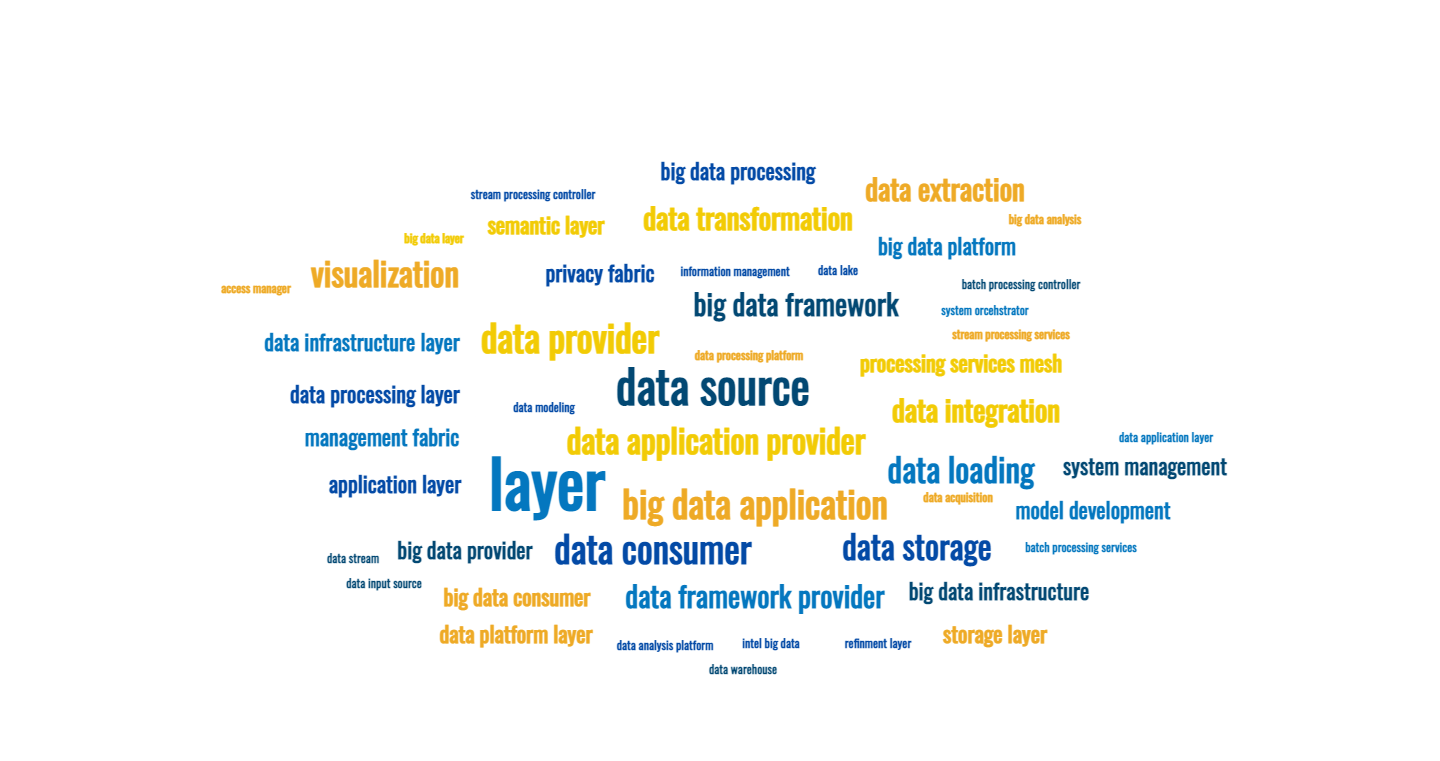
\includegraphics[width=18cm]{wordcloud.png}
    \caption{BD RA Component Names Word Cloud}
    \label{image:word-cloud}
\end{figure*}

Among the names authors used to name their components, 'big data application provider' (5 occurrences), and 'big data framework provider' (3 occurrences) seems to have been used the most. This is due to the fact that some of the RAs are built upon NIST BD RA (s17), and have therefore adopted the terminology. One term that all studies seems to have been using uniformly is 'data consumer' and 'data provider'. Moreover, most studies have chosen the phrase 'layer' to logically group different components of the RA.

Taking all into consideration and to answer RQ2, we paid clear attention to the description of these components and categorized them based on their functions. These categories are; 1) BD Management and Storage, 2) Data Processing and Application Interfaces, 3) BD Infrastructure.

\subsection{BD Management and Storage}

One of the prominent characteristics of big data is ‘variety’, which rises the need for distinct storage solutions. This is sometimes referred to as ‘polyglot persistence’ \cite{khine2019review}. For instance, when it comes to dynamic data, NoSQL databases such as MongoDB is a suitable choice because of their non-tabular nature (Banker, Garrett, Bakkum, \& Verch, 2016), and when there is a need for complex relationship between entities, graph databases such as Neo4J are more suitable because of their tree traversal performance (Van Bruggen, 2014). 
 
Choosing the right database or databases, is an important architectural decision that can also include patterns for data access, storage and caching. For example, the practitioners of distributed system that are specialized in micro-services architecture may opt to use Command Query Responsibility Segregation (CQRS) pattern for high performance event driven applications \cite{marquez2018actual}. The type of storage and the access pattern are two major architectural components of big data systems. 

The current landscape of BD RAs seems to revolve around monolithic storage solutions such as data warehouse and data lake. While the traditional practice of staging data, dimensional modeling, storage in data warehouses, and data marts as customized access layers, may seem ineffective in handling BD loads, we've been surprised to still witness some variations of this approach being proposed.  

Another architectural component that is popular in BD RAs is data lake. Data lake can be perceived as an ingestion framework that can be given various types of data including internal and external data. The data stored in the data lake is then usually retrieved for transformation. This is the LET (load, extract, transform) approach, comparing to old ETL (extract, transform, load) approaches. 

Similar to the way that Business Intelligence (BI) and BD differ in their source data types both in terms of granularity and data structure of it, a data lake and data warehouse are different. In the case of a data warehouse, usually a relational database is used which decreases flexibility when it comes to analysis and can potentially cause considerable costs. In the case of data lake, data of different kind can be stored without the engineer needing to define the schema in advance. This increases the flexibility.

Howbeit, this flexibility itself has its own downside and can be abused by data engineers. One can throw different data sets in the data lake, without much regard for how they’re structured and consumed, and this can in turn, result in the creation of a data swamp. Data governance and active metadata can alleviate some of these issues \cite{monolithToMesh}.

Based on the results of this synthesis, we posit that BD RAs are driven by three main paradigms; 1) enterprise data warehouse paradigm, 2) data lake paradigm, and 3) multi-modal cloud based paradigm. 

The first paradigm revolves around large monolithic enterprise data warehouses, with ETLs, staging environments and a data processing pipeline. A good example of the first paradigm is S5. The second paradigm is about monolithic data lakes containing data that follows a similar data processing pipelines as data warehouses, but happening at a later stage. A good example of the second paradigm is S21. The third paradigm is not that far away from the second, but aims to incorporate more elements of distributed systems and cloud features. A good example of this paradigm is the S22.

Moreover, some RAs sit at a higher level of abstraction. A good example is S20. For these kind of RAs, one cannot assume the nature of the data pipelines and if the storage would be monolithic or not. In S20, there's a depiction of various kinds of storage in the 'Big Data Platform Layer', indicating that one may choose to opt in for polyglot persistance. Therefore, only the resulting system can help us realize what paradigm the RA may belong to. 

When it comes to big data management, many of the cross-cutting concerns seems to be overlooked. For instance, we have realized that many BD RAs do not pay a clear attention to security, privacy, metadata management and data quality. While some RAs tend to revolve around security such as S13, and some other tend to revolve around metadata management such as S15, we could not find a comprehensive explication of BD cross-cutting concerns.

We could not understand how some of the RAs could scale to account for data source proliferation and how rapidly they could react to regional data privacy changes. We could hardly see a discussion on data architecture, data discoverability, and data interoperability.

\subsection{Data Processing and Application Interfaces}

There are two major data processing activities that a BD system encompasses. These processes generally fall into stream processing and batch processing. Stream processing or fast processing is required for sensitive operations and time critical processes such as checking a fraudulent credit card, and batch processing required for a long-running continuum of data analysis such as regression analysis. 

The decision on required type of processing for a context-specific architecture is determined by the characteristics of the data being analyzed, that is primarily variety, volume and velocity. 

For instance, most algorithms for stream processing are using in-memory stateful data structures such Hyperloglog to compute values in real-time. A streaming component can be tailored to adopt specific windowing approaches such as tuple-at-a-time and a micro-batch processing. When in fact, these techniques are not required for batch processing. An architect may opt for MapReduce and Bulk Synchronous Parallel (BSM) processing for batch-oriented requirements or go for a streaming processing based on a specific performance requirement set to handle velocity and volume of data. 

Various studies have provided different level of abstraction when it comes to describing data processing. While some studies like S19 describe the processes in the data processing pipeline, some others like s15 have just abstracted it to 'batch processing' or 'stream processing'. 

Moreover, we realized two category of data processing. First category utilizes two different architectural constructs for batch and stream processing, while the latter tends to process both in one architectural component. That is, one category processes both streaming and batch in one computational unit, while the other separates them. This is a difference that can be seen between Lambda and Kappa, and the RAs that have been derived from the two. Some RAs such as S17 have used three architectural constructs, namely batch node, streaming node and interactive node. 

BD interfaces are communicated in two different ways, either the RA only presented a 'serving or access layer' (S21, S17), or several components that are each specific to a different requirement (ML, BI, etc). The latter can be witnessed in S16.

Some RAs tend to clearly distinguish to ingress and egress interfaces and inter-node interfaces such as s22, while others mostly annotated interfaces with just an arrow. Along the lines, some studies have created terms for their interfaces such as 'provider-request interface' in s15. While interfaces are quite important architectural constructs, current RAs don't seem to be vested a lot of interest in clearly portraying them. 

\subsection{BD Infrastructure}

Another major area that is discussed in the RAs is the concept of infrastructure. Different authors have taken different approaches to communicate this. Some have presented it through a standard architectural description language such as s6, which clearly defines the technology layer, and some have not mentioned the concept of infrastructure, but it's rather implicitly conveyed such as s21 and s22. Some other have presented with both infrastructure and platform layers such as s20 and s17. 

For instance, one major component of a NIST BD RA (s17) is called big data framework provider which includes ‘computing and analytics’, ‘data organization and distribution’, and ‘infrastructures such as networking, computing and storage’.  

BD infrastructure is more of a layer than a component. A layer in which the RA lays out a possible computing and networking design of a BD system. This is crucial, as practitioners of BD have been commonly architecting underlying distributed paradigms and horizontal scaling. 

Therefore, CAP theorem, ACID and BASE transactions, data consistency, service discovery, and tail latency are potential architectural challenges one should consider. Should a BD system adopt an event-driven approach through an event backbone such as Kafka that is discussed in s22? Or should it stick to REST based communication? What is the overhead of context switch and networking among services?  

All and all, as a result of this SLR, a component of a BD infrastructure has been witnessed as a common pattern, in various forms and approaches. We consider platform layer of BD as a major architectural component of these systems. Whereas one might argue that infrastructure is an architectural component of any system, the design challenge is more significant in the case of BD systems as these systems are usually distributed in nature.

Another area that seems to be neglected is DataOps. While DataOps can play an important role in the automation and delivery of data engineering workloads in an agile manner, we could not find BD RAs that incorporate this aspect.

Lastly, our findings depicts the fact that many of RA presented are not designed underlying completely distributed architectures while BD systems can benefit from this paradigm. An exception to this is S22, which is absorbing many patterns from event-driven microservices architecture.

\section{What are the limitations of current BD RAs?}

To answer the RQ3, RAS collected for this SLR have been appraised to point out limitations. To arrive at this objective systematically, we first described each RA with its limitation briefly. This is portrayed in table \ref{table:BD-RAs-Limitations}.


\begin{table*}
    \caption{BD RAs and Their Limitations}
    \renewcommand*{\arraystretch}{1.4}
    \label{table:BD-RAs-Limitations}
    \begin{tabular}{|p{0.3cm}|p{16.8cm}|}
        \hline
        RA & Description/Limitations \\ 
        \hline
        S1 & Lambda architecture, being developed at an early stages of BD hype, does not seem to have an overarching approach to data architecture and several limitations are witnessed. The architecture does not address data quality issues, does not seem to address changes in landscape of data, does not address privacy, security and metadata. This architecture seems to be providing with the bare minimum requirement for BD systems  \\
        \hline
        S2 & This RA is specifically designed for the domain of healthcare and life sciences, does not seem to account for data quality, security and privacy. Resembles to monolithic n-tier architectures, and pivots on IBM specific solutions such as LSF process manager, LSF application center, and LSF data manager. There is no notion of data accountability and interoperability. \\
        \hline
        S3 & This RA seems to be covering a very general scenario of big data analytics, without any attention to either metadata or security. It flows from data sources to data transformation, and into data usage, but it's unclear how data quality is assured, how it will support changes in data landscape, and how it will respond to changes. In addition, the RA is heavily influenced by MapReduce, while MapReduce may not provide the best of performance in comparison to newer approaches such as acyclic direct graph used in Apache Spark and Tez.  \\
        \hline
        S4 & A classically designed RA with 3 main phases of ingestion, processing and providing. This RA has underlying mechanisms that facilitates 'right-time' flow of data through the system. This is achieved by having two architectural constructs for strongly typed data and weakly typed data. While this was annotated as the data quality part of the RA, it does not seem to account for data ownership and changes in data landscape. In addition, this RA utilizes data mart for access and performance, which can affect the overall modifiability negatively. In addition, we could not tell how data governance takes place.  \\
        \hline
        S5 & This RA is the augmentation of traditional data warehouse architectures with a few new components to account for stream processing. There seems to be many moving parts in this RA, and privacy and metadata is clearly addressed. Nevertheles, the RA is lacking in the area of security, data provenance, scalability and modifiability. We can't tell how data ownership is in place, and how data quality is addressed. \\
        \hline
        S6 & This RA seems to be portraying the bare minimum requirements for big data analytics with no mention of security, privacy, metadata, or data quality. The RA is published as a short paper, thus not much detail is given. \\
        \hline
        S7 & This RA provides with bare minimum components for data analytics, without any clear identification of stream processing. The RA seems to be done in quite a reductionist manner, with no attention to privacy, security, metadata, and data quality. Data storage seems to be only associated to hardware, and thus it's unclear how data is evolved and scaled.  \\
        \hline
        S8 & Kappa is perhaps the predecessor of Lambda, aiming to address some of the limitations of it. The major difference between Kappa and Lambda is that Kappa has a unified processing layer for batch and stream process, which eliminates the complexity of maintaining two separate systems, and reduces costs. Nevertheless, this architecture, does not discuss metadata, security, privacy, data quality, and maintainability in details.  \\
        \hline
        S9 & This BD RA is designed for healthcare application by Intel. This RA is not elaborated in detail, does not seem to account for cross-cutting concerns such as security, metadata, privacy, and data quality. The concept of access manager seems to be vague, as we could not understand how the access is managed. The artefact seems to be a simple instance of Hadoop ecosystem with some extra components added   \\
        \hline
        S10 & A comprehensive RA that aim to cover many aspects of data engineering. Nevertheless, we did not find any notion of metadata management, neither was a discussion on security and privacy challenges. While this RA could work successfully for a regular BD workflows, we are unsure how data quality is met and how scalability is achieved.  \\
        \hline
        S11 & This RA is made up of three major phases, ingestion, processing and presentation. It is designed around Hadoop ecosystem, and provides with bare minimum necessary to conduct data analytics. We could not find a discussion on metadata management, security, privacy or data quality. The data pipeline is using a data warehouse,and uses it to communicate to the Hadoop side of things. We are not sure how unstructured data is handled, and how data lineage is achieved.  \\
        \hline
        S12 & This architecture is specifically designed for waste management, and seems to be using an approach similar to Kappa. The data takes a generic flow from data sources to application, without any clear identification of data quality, privacy and security concerns.    \\
        \hline
        S13 & This RA is specifically deigned for the security domain and seems to have a lot of inspiration from NIST BD RA. The RA is layed out in fabrics just like the NIST one, and unlike many others, does mention cross-cutting concerns such as security explicitly. However the concept of data ownership is not discussed, there's no mention of metadata or privacy, and the artefact evaluation is not extensive. That is, we cannot ensure how the derived solutions from this RA can scale.    \\
        \hline
        S14 & A generic RA that resembles to Lambda architecture, with stream and batch processing being processed in different nodes. This RA utilizes data warehouses and hadoop cluster for data processing. It was unclear how the security, privacy, metadata, and data quality is achieved. Maintainability aspects are not discussed as well. \\
        \hline
        S15 & This RA extends the Lambda architecture by adding a semantic layer. It has a great focus on handling metadata in a right manner, but it does not seem to have any identification of other cross-cutting concerns such as privacy, security or data quality. It also adopts the idea of separate batch and stream layers, which can potentailly affect modifiability negatively and increase cost. \\
        \hline
        S16 & This RA clearly segregates stream data from other data, and defines clear interfaces for ingestion of different data types. It then passes the data directly to a distributed storage (Hadoop's HDFS), and retrieves it later for deduplication and cleaning. While the RA seems to have addressed the minimum requirements of data analytics, it does not seem to address cross-cutting concerns such as metadata, security and privacy. It is also unclear how data quality is achieved. \\
        \hline
        S17 & This is perhaps the most comprehensive BD RA found in this SLR, and has been heavily funded by the government of the USA. While this RA is a good tool to facilitate open discussion, design structures, requirements, and operations inherent in BD, it is more of a high-level conceptual model of BD, rather than an effective BD RA. Some of the limitations witnessed in this RA is in its brief mention of metadata management (only discussed in lifecycle management), unclear approaches to attain data quality and data ownership, and potential monolithic coupling of components in big data application provider. \\
        \hline
        S18 & This RA segregates data extraction and data loading phases, and tend to adopt the idea of segregating stream and batch processing layers. Nevertheless, we could not find the identification of cross-cutting concerns such as privacy, security or metadata management. We could not understand how data quality is achieved. There are also three storages designed, but seems like all data will eventually be stored in one giant storage. This can potentially make modifiability harder and create a choke point. \\
        \hline
        S19 & Driven from the NIST BD RA, this RA is more ore less identical with BD RA, but tailored specifically for emergency management. We skip explanation for this RA, as the limitations discussed for NIST BD RA, can be applied to this one as well. \\
        \hline
    \end{tabular}
\end{table*}

\begin{table*}
    \renewcommand*{\arraystretch}{1.4}
    \begin{tabular}{|p{0.3cm}|p{16.8cm}|}
        \hline
        S20 & This RA shares all the fundamental components with NIST BD RA, and seems to be very similar. However, the phrase fabrics seems to be changed to multi-layer functions. Therefore this RA, just like NIST is too abstract and leaves many architectural decisions unknown such as data storage, data quality assurance, and data ownership. It is unclear on how storage should be approached, and the overall structure resembles to a monolithic data pipeline architecture. \\
        \hline
        S21 & One of the few RAs that tend to absorb the concept of microservices into BD development. Nevertheless, the RA seems to be driven by the idea of one data lake for all data storage, which can be a daunting task to scale and maintain. The concept of metadata does not seem to be discussed, and other concerns such as security, privacy, data quality and data provenance are unclear.  \\
        \hline
        S22 & This RA absorbs a lot of patterns from microservices event driven architectures and reactive systems and tend to absorb them into the BD development. While there's been a clear attention to cross-cutting concerns such as metadata, and privacy, security does not seem to be well discussed in the study. The RA also tends to use data lake as the single source of storage which can be challenging to scale.  \\
        \hline
    \end{tabular}
\end{table*}

Except for one case (S22), all the architectures and RAs found as the result of this study, were designed underlying monolithic data pipeline architecture with four major components being data consumer, data processing, data infrastructure and data providers. To discuss the integral facets that embroil these architectures, one must look at the characteristics of these architectures and the ways in which they achieve their ends.

The process of turning data into actionable insights in these architectures usually follow a similar lifecycle;

\begin{enumerate}
    \item \textbf{Data Ingestion}: system begins to ingest data from all corners of the enterprise, including both transactional, operational and external data.
    \item \textbf{Data Transformation}: data captured from the previous step is then cleansed for duplication, quality, and potentially scrubbed for privacy policies (scrubbing is hardly discussed in the studied RAs). This data then goes through a multifaceted enrichment process to facilitate data analysis.
    \item \textbf{Data Serving}: at this stage, data is ready to be served to diverse array of needs ranging from machine learning to marketing analytics, to business intelligence to product analysis and customer journey optimization.
\end{enumerate}

The lifecycle depicted is indeed a high-level abstract view of prevalent BD systems. Howbeit, it highlights an important matter; these systems are all operating underlying monolithic data pipeline architecture that tends to account for all sorts of data. This means, data that logically belong to different domains are now all lumped together and crunched in one architectural constructs, making maintainability and scalability a daunting task.

While architectures in software engineering have gone through series of evolution in the industry, adopting a more decentralized and distributed approaches such as microservice architecture, event driven architectures, reactive systems, and domain driven design , the data engineering, and in specific BD ecosystems do not seem to be adopting many of these patterns. The whole idea of 'monolithic data
pipeline architecture with no clearly defined domains and ownership' brings significant challenges to design, implementation, maintenance and scaling of BD systems.

This architecture and system design if done underlying these approaches, can result in hard to maintain systems with high costs, and leave many managers disappointed. Nevertheless, we don't claim that all these architectures will fail, perhaps some have proven to be successful in a specific context. There are two threats to maintainability and scalability of these systems; 

\begin{itemize}
    \item \emph{Data source proliferation}: as the BD system grows and more data
    sources are added, the ability to ingest, process, and harmonize all these data in one place diminishes.
    \item \emph{Data consumer proliferation}: organizations that utilize rapid experimentation approaches such Hypothesis-Driven Development and Continuos Delivery constantly introduce new use cases for data to be consumed in different domains. This means that variability of the data rises, and the sum of aggregations, projections, and slices increases, which in turn adds more work to the backlog of the data engineering team, slowing down the process of serving the data to consumers.
\end{itemize}

Another limitation that we came across was that the concept of metadata has been poorly discussed. For instance, s5 discussed the limitation of metadata management systems, stating that most metadata solutions are ad-hoc. The researcher then went ahead and introduced a layer for metadata management in the RA, but as a non-integrated component. For instance, the author did not discuss how data provenance can be achieved through the RA and underlying which logical flow one can do linear analysis. 

In another case, NIST BD RA only discusses metadata in a sentence, and in sub-activity named ‘metadata management’. The RA only states what are essential metadata information and how they are used. Except for s15 and s22, metadata has not been accentuated enough and metadata layer is not thoroughly discussed. This is a noticeable limitation in current BD RAs, as metadata plays an important role in BD systems, addressing wide range of challenges such as privacy, security, data provenance, data lineage and linear analysis. Practitioners of BD systems are now working on large-scale metadata systems such as metadata lake.

Based on that, one can argue that any BD system can benefit from a well-defined metadata layer as a means for bridging data stored in different platforms such as on-premises or on cloud, reducing complexity, facilitating access management, facilitating data governance, and potentially the creation of data mesh.

Furthermore, white papers collected from IT giants tend to pivot the RA around their services, which can potentially reduce its applicability, hinder RAs openness, and even affect architectural qualities. In these white papers, alternative technologies or vendors are typically not discussed which leaves the architect with a small pool of options.

Lastly, privacy and security do not seem to have been discussed enough, or it has been mostly marginalized. For instance, we have not found an architectural component that allows for data scrubbing, or we did not understand how one can achieve security in-between data pipelines. Specially, in regard to privacy and with recent global movements towards increased privacy, BD architects are now increasingly challenged to design under the shadow of regional data privacy policies such as GDPR. Placing this challenge next to security challenges of package management, endpoint proliferation and DDOS handling can further signify the necessity for more research on BD RAs.

Many of core architectural decisions revolving around security and privacy, if not addressed in an initial phase, can result in massive losses and potential bottlenecks. 

\section{Discussion}

In this section, we provide a summary of main findings and the potential implications for both industry and academia. 

In this study, by adopting a rigorous research methodology, we aimed to understand the state of the art in BD RAs. To the best of our knowledge, there is no study in academia that has conducted a SLR on BD RAs, nor there is a systematic mapping study. While RAs can play a pivotal role in development and maintenance of BD systems, there does not seem to be enough attention on this topic. 

The closest study we could find to comparing and analyzing BD architectures was the work of Volk et al (\cite{volk2019decision}), which does not revolve around BD RAs, but attempts to develop a decision support system for selecting BD reference architectures. However, this study stays fairly light on BD architectures and does not aim to systematically collect them. 

The researchers of NIST BD RA (S17) have collected a series of white paper from the big data public working group, and used it as a foundation study. Howbeit, these white papers are not detailed BD RAs, and are mostly proof of concepts that different members of the group have put together for the purposes of contrast and comparison. 

Our findings from this study yielded the fact that progress is uneven in the area of BD RAs. While there are many researches in the area of data warehousing, artificial intelligence, data science, and IOT, data engineering seems to be needing more research. While, there are many well established approaches for crunching large volume of data, or handling dimensionality of complex data sets, the overall organization of BD technologies, which is the architecture, needs more attention from academia and industry. 

Majority of the BD RAs that we have analyzed were running underlying some sort of a monolithic data pipeline with a central storage. This is a challenging architecture to scale and maintain. How does one takes preventive measures to stop a data lake from turning into a data swamp ? How a team of hyper-specialized siloed data engineers that are running the data pipelines, will be aware of the actual consumption of the data and therefore keep a certain level of quality of that data? how data interoperability is achieved? how data ownership is institutionalized ?

If a software engineers decides to, for instance, manipulate a certain field in a certain entity's schema for the development of a new feature, how will this affect the data engineering process and how is this communicated? as data becomes more and more available to the company, the ability to consume it all in one place diminishes. 

On the other hand, the current state of BD RAs do not seem to be very far away from traditional data warehousing approaches. In fact, some of them have adopted the idea of data marts and propose them as BD solution, but using newer technologies. Moreover, some architectures have attempted to utilized datagit lake to serve data analysts and business intelligence. 

We posit that neither the attempt to onboard BD analytics workloads to data warehouses, nor the attempt to serve business intelligence with data lakes is gonna result in a scalable and maintainable system. We therefore propose the need for future research directions in the area of decentralized and distributed BD RAs. 

We also felt that the quality of many of BD RAs published does not seems to be enough to meet the industrial expectations. This is due to the challenges of developing BD RAs and the cost and resources required to evaluate these artifacts. It is also worth mentioning that a rigorous methodology for evaluating reference architectures are quite rare, and while there are studies that have attempted to address these issues (\cite{angelov2008towards}), there is a need for more research in this area.

Given all, we posit that RAs can be considered an effective initial point to design and development of BD systems. These artifacts helps facilitating communication, capture requirements from various stakeholders, and catch design issues while they are still cheap. Based on this, therefore, more and more attention needs to be given to this area and its foundational methodological needs. 

\section{Threats to Validity}

Just like any rigorous SLR, and based on our research methodology, it is essential to conduct a 'threats to validity' assessment to transparently communicate any bias or flaws that research may suffer from. Therefore, the threats to validity for this study are as following;

\begin{enumerate}
    \item \emph{Construct Validity}: This SLR is as good as the quality of the evidence collected and the synthesis of it. Therefor we have taken extensive measures to maximize the rigour in this study. By following some of the most prominent guidelines for SLRs, and a few complementary studies for search strategy, inter-rate reliability, data synthesis, and quality assessment, we ensured that at every step we are removing bias, and increase transparency and systematicity of our study. We also opted for thematic synthesis, and followed a well established approach to create themes and models.
    \item \emph{Internal Validity}: To avoid losing on valuable information, we augmented our SLR with grey literature, and used a rigorous method to incorporate those literature into the main pool of literature. We snowballed papers, looked for references, and even searched the works of well-known researchers in the field. 
    \item \emph{Conclusion Validity}: One potential threat to validity might be that some of the studies we collected may not have been mature enough, and that in turn might have impacted the generalizability of our conclusions. To mitigate this threat, we have developed a rigorous quality framework and assessed each pooled literature based on it. We made sure that this process is conducted by different individuals so to achieve the quality desired. 
\end{enumerate}

\section{Conclusion}

This study sought to find all BD RAs available in practice and academia. The findings gained emerges the understanding that RAs can be an effective artefact to tackle complex BD system development. RAs at their core bring software engineering knowledge as a collection of patterns designed to address a class of problems with attention to specific requirements and context and do solve many of the prevalent architectural challenges that an architect might face. 

As data proliferates further, there will be more BD systems created which in turn means more technology orchestration is required around data that can be effectively done through a well-established RA. RAs guide the evolution of the system both in terms of functional and non-functional requirements, and pinpoint variability points that can result in more successful BD projects and avoidance of common pitfalls. 

Withal, BD RAs have yet to mature and become ubiquitous in industry and there is further research required in this area. These researches can be done in the area of micro-services RA for BD systems, event-driven paradigms for BD systems, security and privacy issues in BD systems, and metadata management.

\bibliographystyle{unsrt}
\bibliography{mybibfile}


\begin{IEEEbiography}[{
\includegraphics[width=1in,height=1.25in,clip,keepaspectratio]{Biography/Pouya-Ataei.jpg}}]{Pouya Ataei} received two bachelor's degree in software engineering from Asia Pacific University, Kuala Lumpure, Malaysia and Staffordshire University, Stoke-On-Trent, The United Kingdom and a master's degree in software engineering from Staffordshire University, is a current PhD student at Auckland University of Technology, Auckland, New Zealand, working on decentralised and distributed big data architectures. He has been an active researcher in the domain of big data within the past 5 years, having created the Nexus methodology for big data system development, and NeoMycelia, a decentralised software reference architecture for big data systems. His area of interest is in distributed system, in specific even driven microservices, reactive systems, software architecture, and data engineering. \end{IEEEbiography}
 
\begin{IEEEbiography}[{
\includegraphics[width=1in,height=1.25in,clip,keepaspectratio]{Biography/Alan-Litchfield.jpg}}]{Alan Litchfield} Dr Alan T Litchfield is Director of the Service and Cloud Computing Research Lab (SCCRL), at the Auckland University of Technology (AUT). He is a partner in a consulting firm that provides specialised services to corporates, government departments and military, is President of the Association for Informa- tion Systems (AIS) Special Interest Group on Philosophy in Information Systems, founding Programme Leader for the Master of Service Oriented Computing (MSOC), member of the AUT Programmes and Academic Review Commit- tee (PARC). Dr Litchfield is member of the Institute of IT Professionals (MIITP), Institute of Electrical and Electron- ics Engineers (IEEE), Association for Computing Machin- ery (ACM), International Institute for Information Design (IIID), TeX Users Gr
\end{IEEEbiography}

\EOD

\end{document}
